\chapter{项目设计与实现}
在本次项目中,我们的项目主要分为两大部分,客户端和服务器端。

客户端可以分为两大部分,前台和后台,前台是安卓界面的显示,后台是创建IPV6套接字,数据的封装与解封装,以及与4over6隧道服务端的通信。
本次项目中的客户端整体流程如图4.1所示:
\begin{figure}[!ht]
	\begin{center}
	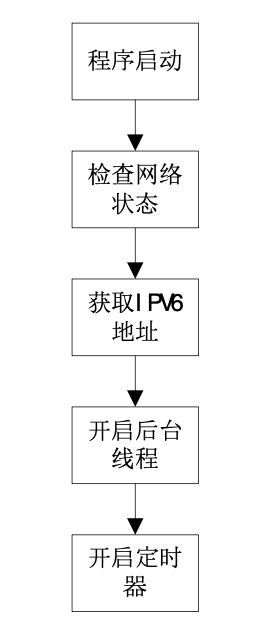
\includegraphics[scale=.58]{client_all.png}
	\end{center}
	\caption{客户端整体流程}
	\label{figure:客户端整体流程图}
\end{figure}

\begin{itemize}
  \item 程序启动后,先检查网络状态
  \item 获取IPV6地址
  \item 开启后台线程
  \item 开启前台定时器刷新界面(间隔1秒)
\end{itemize}

前台是java语言的显示界面,后台是C语言的数据交互,前后台之间通过管道进行通信,这里创建了两个管道,一个是IP信息管道,一个是流量信息管道,两个管道分开处理相对简单,通信的详细流程如图4.2下所示:
\begin{figure}[!ht]
	\begin{center}
	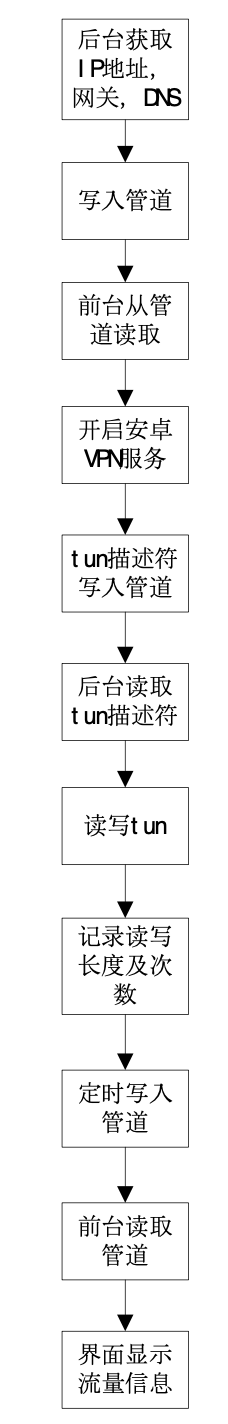
\includegraphics[scale=.58]{front_back.png}
	\end{center}
	\caption{前后台通信流程}
	\label{figure:前后台通信流程图}
\end{figure}

\begin{itemize}
  \item 后台获取到4over6服务器发送来的IP地址等信息
  \item 把这些信息解析出来,写入IP信息管道
  \item 前台从IP信息管道读取到IP地址等信息
  \item 开启安卓VPN服务
  \item 把安卓虚接口描述符写入IP信息管道
  \item 后台从IP信息管道获取安卓虚接口文件描述符
  \item 对该虚接口进行读写操作
  \item 记录读写长度和次数
  \item 在后台定时器线程,定时写入流量信息管道
  \item 前台从流量信息管道获取流量信息
  \item 定时刷新界面的流量信息
\end{itemize}

服务器端主要可以分为三部分:主进程循环、读取虚接口线程、keeplive线程。主框架流程图如图4.3下所示:
\begin{figure}[!ht]
	\begin{center}
	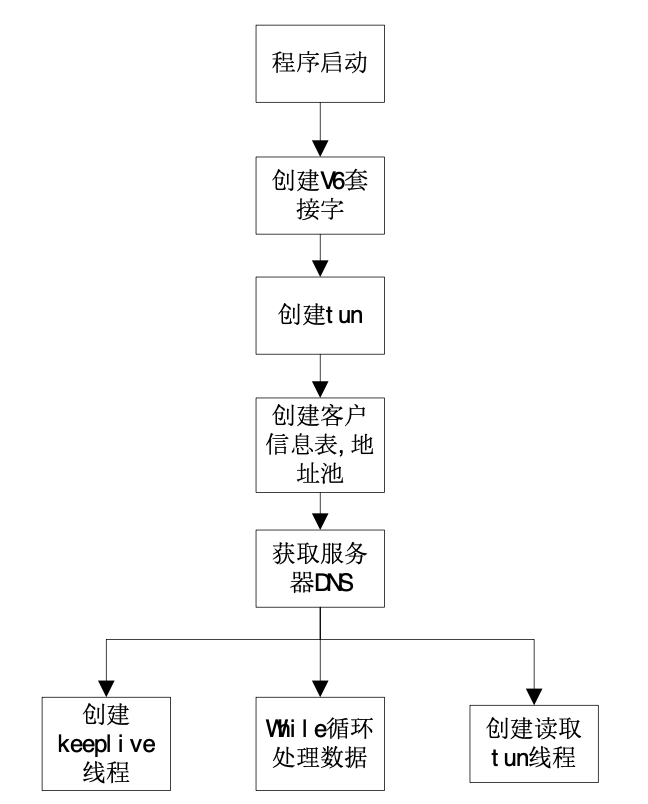
\includegraphics[scale=.58]{server_all.png}
	\end{center}
	\caption{服务器端整体流程}
	\label{figure:服务器端整体流程图}
\end{figure}

\begin{itemize}
  \item 创建IPV6套接字,把该套接字加入Select模型字符集
  \item 创建tun虚接口
  \item 创建客户信息表和地址池
  \item 获取服务器DNS地址
  \item 创建keeplive线程
  \item 创建读取虚接口线程
  \item 主进程中while循环中数据处理
\end{itemize}

\section{客户端前台流程设计}
\begin{figure}[!ht]
	\begin{center}
	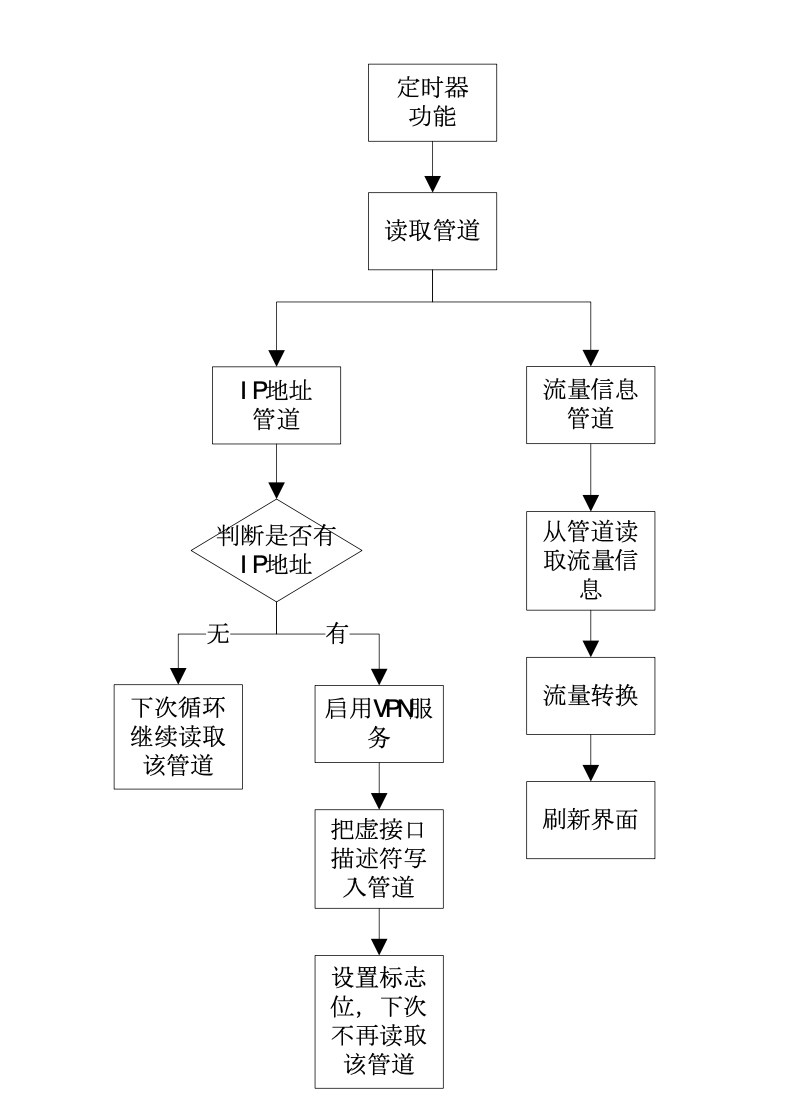
\includegraphics[scale=.58]{front.png}
	\end{center}
	\caption{客户端前台流程设计}
	\label{figure:客户端前台流程设计}
\end{figure}
前台的详细流程图如图4.4所示,前台定时器主要功能为定时刷新显示界面,显示流量信息,定时器功能解析如下:
\begin{itemize}
  \item 开启定时器之前,创建一个读取IP信息管道的全局标志位flag,默认置0
  \item 开始读取管道,首先读取IP信息管道,判断是否有后台传送来的IP等信息。假如没有,下次循环继续读取
  \item 有IP信息,就启用安卓VPN服务
  \item 把获取到的安卓虚接口描述符写入管道传到后台。把flag置1,下次循环不再读取该IP信息管道
  \item 从管道读取后台传来的实时流量信息,把流量信息进行格式转换并显示到界面
  \item 界面显示的信息有运行时长、上传和下载速度、上传总流量和包数、下载总流量和包数、下联虚接口V4地址、上联物理接口IPV6地址
\end{itemize}


\section{客户端前台具体实现}

\subsection{UI主界面}
主界面采用了 ScrollView 嵌套 LinearLayout 的布局方式,将连接 VPN 前后的不同界面通过一个 Layout 展示,通过控制不同组建的可见显示,实现界面的切换。程序界面主要分为 连接VPN前 和 连接VPN后 两个部分。

程序启动时主界面属于连接VPN前界面。其包含两个可输入窗口,分别用于动态设置服务器 IPV6 地址以及服务器端口号。另一个展示栏显示当前本机连接状态以及本机 IPV6 地址。另外两个按钮分别实现连接 VPN 功能以及退出程序功能。当本机网络环境满足需求时,即处于 IPV6 网络环境,可以通过点击【连接 VPN】跳转到连接信息展示界面,此时隐藏初始界面的元素,并将信息展示界面元素显现以实现页面转换。 

连接前程序界面如图4.5所示:
\begin{figure}[!ht]
	\begin{center}
	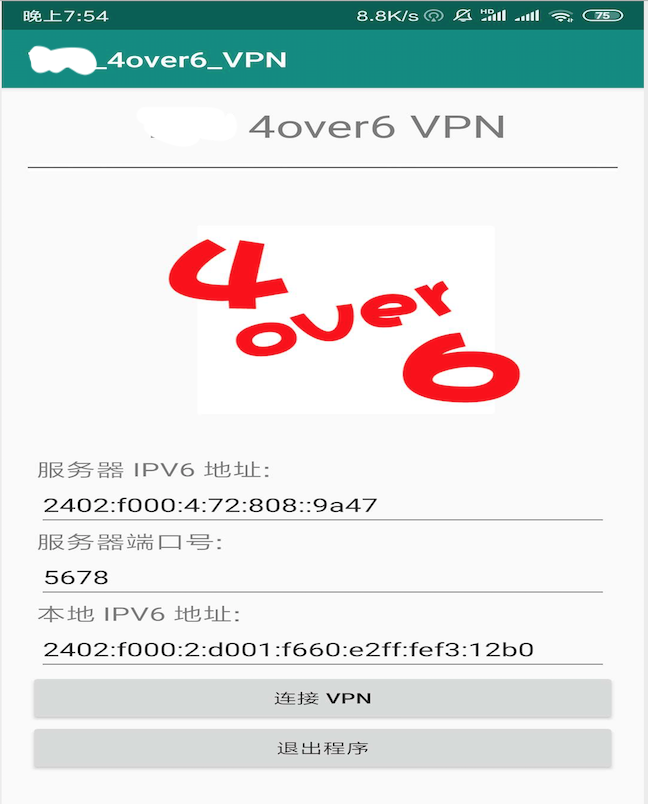
\includegraphics[scale=.58]{connect1.png}
	\end{center}
	\caption{连接前程序界面}
	\label{figure:连接前程序界面}
\end{figure}

连接VPN后 的界面可以展示当前程序运行时间,本机分配的 IPV4 地址,上网速度,总共接收发送包大小等信息。一个【断开 VPN】按钮可以将本机与服务器断开,并回到初始化的界面。

% 连接后程序界面如图4.6所示:
% \begin{figure}[!ht]
% 	\begin{center}
% 	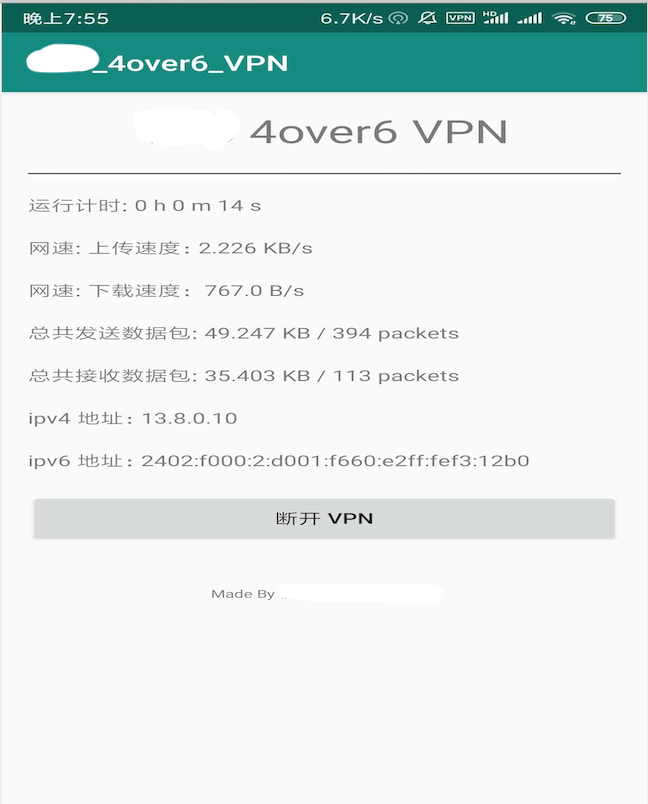
\includegraphics[scale=.58]{connect2.png}
% 	\end{center}
% 	\caption{连接后程序界面}
% 	\label{figure:连接后程序界面}
% \end{figure}

\subsection{MainActivity}
MainActivity 是本程序的主线程,其主要完成程序的初始化工作,以及启动多个线程以支持程序工作。当程序启动时,MainActivity 首先完成对于界面的初始化,为按钮注册监听事件,并每隔 2s 检查本机的网络环境,调用 NetChecker 的 getIpv6Address 尝试获取本机的 IPV6 地址。只有成功获取了本机的 IPV6 地址,才能继续后续的 VPN 服务。

当点击【连接 VPN】按钮后,首先检查是否允许开启 VPN 服务,满足条件会启动 C 后台线程以及前端的定时器线程。C 后台线程见后端具体实现。

前端的定时器线程同前述工作流程。首先连接 IP 信息的管道,接收 C 后台线程传来的 IPV4 地址,DNS 等信息,然后启动 VPN 服务。通过继承 java.util.TimerTask 实现连接 C 后台线程创建的流量信息管道,读取信息并实现 UI 界面信息的更新。 

当点击【断开 VPN】按钮后,会结束 C 后台线程以及前端的定时器线程。

\subsection{MyVpnervice}
MyVpnService 是一个继承了 VpnService 的类,其与主线程 MainActivity 之间通过 Intent 进行数据交换。其需要完成的主要功能是:根据传入的 IPV4 地址,DNS 服务器等参数,初始化 VPN发 服务,并尝试获取虚接口的文件描述符。当获取描述符后,通过管道将数据传给 C 后台。
\subsection{NetChecker}
NetChecker 类主要实现调用 Android 接口,检查本机当前网络环境,并尝试获取 IPV6 地址的功能。isWIFIConnected 负责检查 Wifi 连接状态,getIpv6Address 负责获取本机 IPV6 地址。主线程 MainActivity 只有通过了 NetChecker 类成功获取到本机的 IPV6 地址,才允许前端开启 VPN 服务。 
\section{客户端后台流程设计}
后台流程图如图4.6所示,详细流程解析如下:
\begin{itemize}
  \item 创建IPV6套接字
  \item 连接4over6隧道服务器
  \item 开启定时器线程(间隔1秒)
  \item 发送消息类型为100的IP请求消息
  \item while循环中接收服务器发送来的消息,并对消息类型进行判断
\end{itemize}

\begin{figure}[!ht]
	\begin{center}
	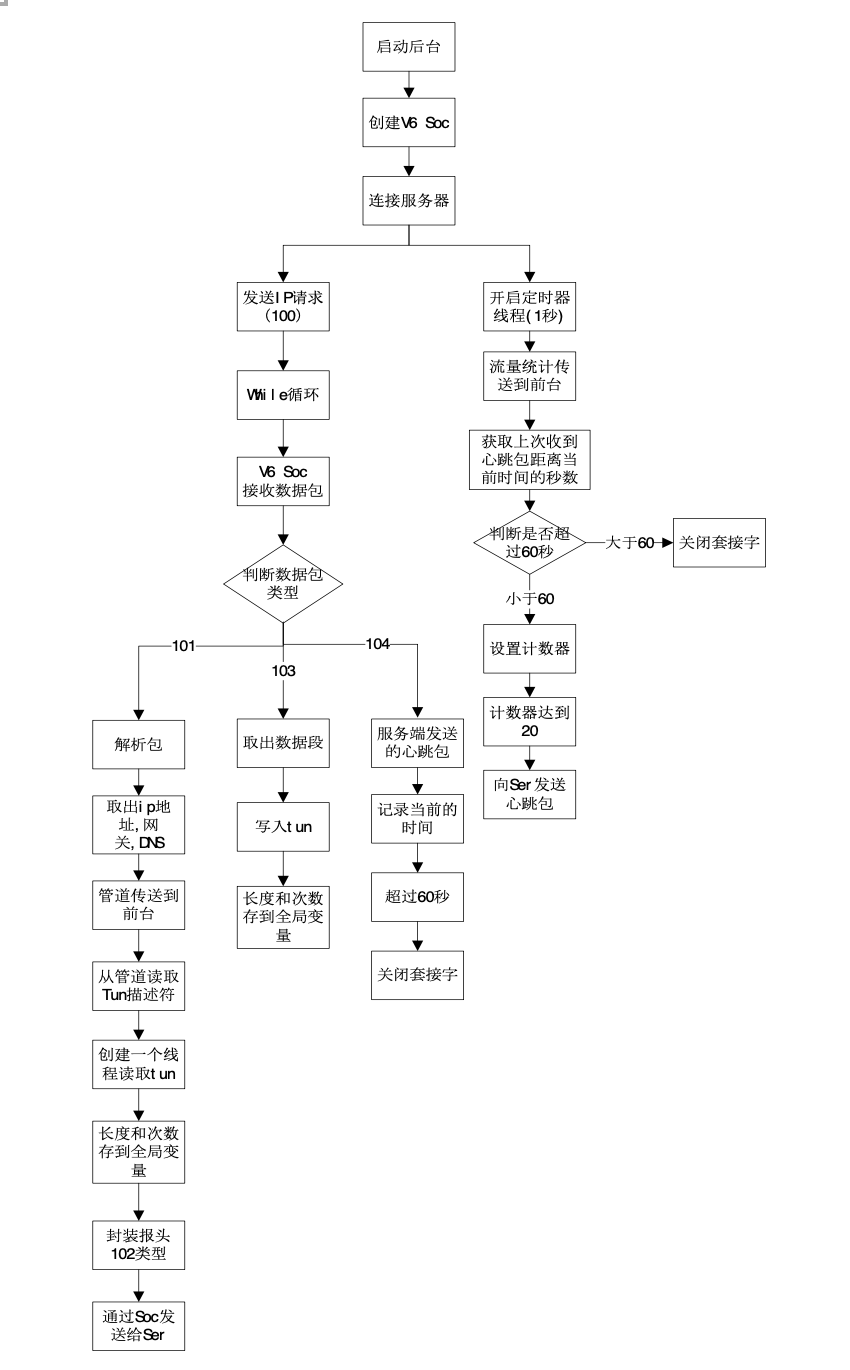
\includegraphics[scale=.58]{back.png}
	\end{center}
	\caption{客户端后台流程设计}
	\label{figure:客户端后台流程设计}
\end{figure}


\section{客户端后台具体实现}
\subsection{JNI}
本次项目需要用 java 代码调用 C 代码,就要用到 JNI。Java Native Interface(JNI) 规定了一套 Java 的原生接口,它提供了若干的 API 实现了 Java 和其他语言的通信(主要是 C和C++)。JNI 是为了本地已编译语言,尤其是 C 和 C++ 而设计的。其支持一个“调用接口”(invocation interface),它允许把一个 JVM 嵌入到本地程序中。本地程序可以链接一个实现了 JVM 的本地库,然后使用“调用接口”执行 JAVA 语言编写的软件模块。
\subsection{后台线程}
当前端启动 C 后台线程时,会传给后台线程服务器的 IPV6 地址以及端口号信息。后端首先进行初始化工作,并建立虚管道,同时使用已有信息创建客户端 Socket,绑定服务器地址,与服务器并进行 TCP 连接。当连接成功时,开启定时器线程 timer\_thread,同时构建 IP 地址请求包,主线程进入 While 循环接收服务器发送来的消息,并对消息类型进行判断,处理数据包。

定时器线程每秒钟会执行一次操作。其主要负责检查与服务器连接是否超时(60s),如果超时则退出 VPN 服务。另外将与服务器连接的相关流量信息(发送/接收包大小,数量)写入管道,并发送至前台,方便前台进行 UI 界面信息的刷新。同时负责每隔 20s 向服务器发送一次心跳包。

主线程在发送 IP 地址请求包后便会进入循环等待并处理服务器发来的数据包。收包的过程是:先构建并清空一个读取缓存 Buffer,首先读取前 4 个字节,代表整个数据包的长度,然后将长度减去 4 之后,按每次一个字节的顺序,逐次读入缓存 Buffer 中,待读取完毕后,将整个 Buffer 拷贝给 Message 即可。根部 Message 的 type 分类,总共需要处理的包有三类(IP地址回应包、上网回应包、心跳包),以下依次讲解:

\begin{itemize}
  \item IP 地址回应包:客户端收到服务器发来的 IP 地址回应包,说明与服务器连接成功。此时需要将数据包中内容(IPV4 地址,DNS 等)经由管道发送给前端,以开启 VPN 服务。完成上述工作后,开启连两个新的线程,一个线程负责循环读取 tun 文件中内容,构造上网请求包发送给服务器;另外一个线程负责持续监听前端是否发来了结束 C 后台线程的指令,以方便结束后台所以运行的线程
  \item 上网回应包:当收到服务器发来的上网回应包时,首先需要统计数据包信息,更新和服务器流量变化,同时需要将数据包内容写入 tun 文件。其中在更新信息时,需要进行加锁操作,实现数据在不同线程间的同步互斥
  \item 心跳包:当收到服务器发来的心跳包,只用更新心跳包收到时间即可,其心跳包发送由定时器线程完成
\end{itemize}

\section{服务器端流程设计}

\subsection{主进程循环}
主进程while循环中主要是Select模型监听所有套接字,然后根据套接字收到数据类型,做不同的处理。while循环如下:
\begin{itemize}
  \item 在while循环中,启用Select模型,对所有的套接字进行监听
  \item 假如监听到服务器套接字,accept新的连接,把新连接的客户端的套接字描述符加入Select字符集
  \item 假如是客户端套接字,首先用ioctl函数判断一下该描述符
  \subitem 假如nread不等于0,客户端正常连接:
    \begin{itemize}
      \item 接收数据
      \item 对收到的数据解封装
      \item 判断数据类型
    \end{itemize}
  \subitem 假如nread等于0,客户端已经断开:
    \begin{itemize}
      \item 遍历客户信息表
      \item 从信息表中查找该客户端描述符所在节点
      \item 取出该节点的IPV4地址
      \item 用该地址与地址池中地址进行匹配
      \item 匹配成功,就把地址池中该地址的标志位置0
      \item 在客户信息表中把该节点删除
      \item Select字符集中清除该描述符
    \end{itemize}
\end{itemize}

while循环流程如图4.7所示:
\begin{figure}[!ht]
	\begin{center}
	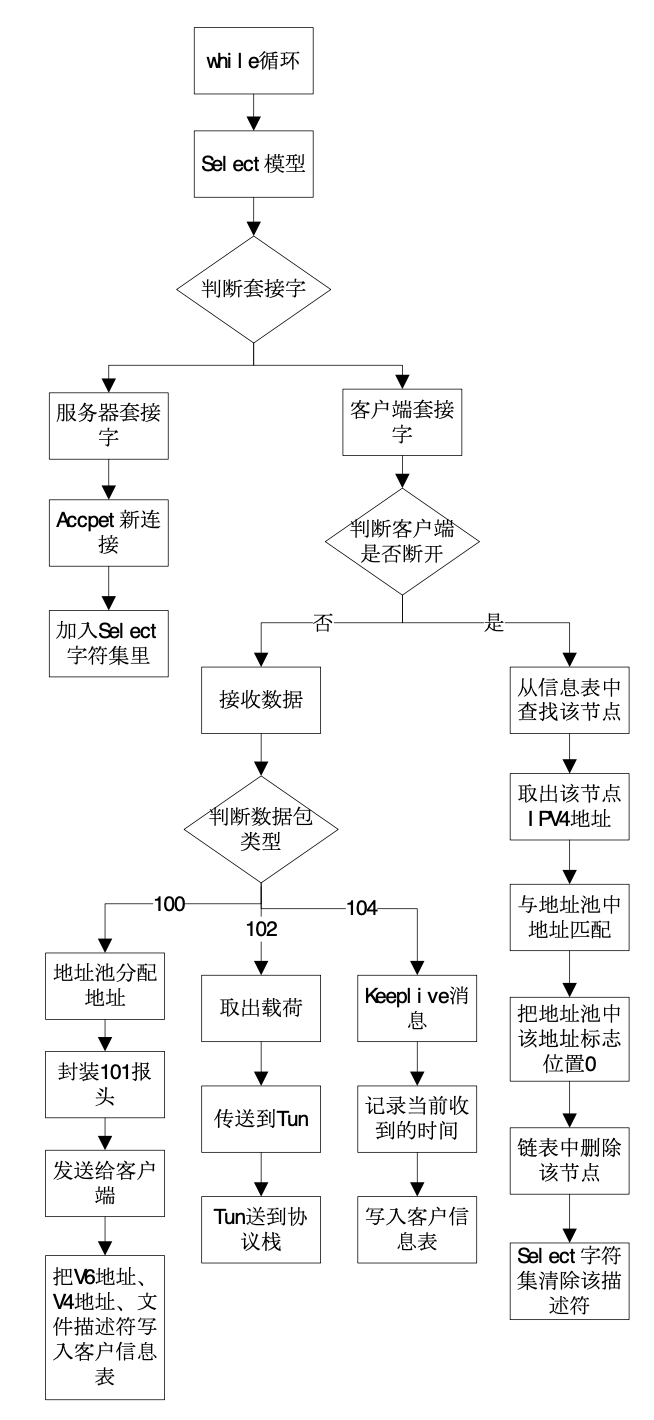
\includegraphics[scale=.58]{server_main.png}
	\end{center}
	\caption{主进程循环流程设计}
	\label{figure:主进程循环流程设计}
\end{figure}

\subsection{读取虚接口线程}

读取虚接口线程主要功能是从协议栈读取消息,根据消息的目的地址,发送给相应的客户端,主要功能如下:
\begin{itemize}
  \item 在while循环中,从虚接口读取消息
  \item 取出该消息的ip头,获取目的ip地址
  \item 遍历客户信息表,查找该目的ip所在的节点
  \item 取出该节点的套接字描述符
  \item 把从虚接口读取到的消息封装103(上网回应)报头
  \item 通过刚才查找到的套接字描述符发送给相应的客户端
\end{itemize}

读取虚接口线程流程如图4.8所示:
\begin{figure}[!ht]
	\begin{center}
	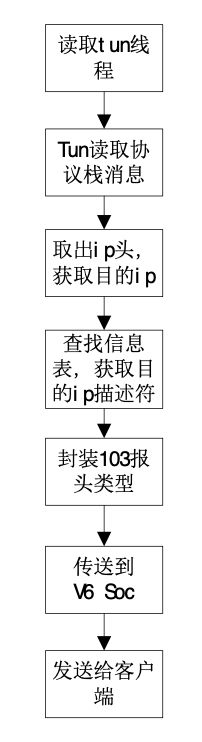
\includegraphics[scale=.58]{server_virtual.png}
	\end{center}
	\caption{读取虚接口线程流程设计}
	\label{figure:读取虚接口线程流程设计}
\end{figure}

\subsection{keeplive线程}
keeplive线程主要功能是给所有当前处于连接状态的客户端发送心跳包,主要功能如下:
\begin{itemize}
  \item sleep一秒钟
  \item 遍历客户信息表
  \item 链表中的每个节点的count字段减1
  \item 当该节点的count字段等于0时,获取该节点的套接字描述符
  \item 通过套接字描述符向该节点所在客户端发送104(心跳包)类型消息
  \item 发送完成,重新把该节点的count字段赋值为20(每隔20秒发送一次心跳包)
  \item 判断每个节点的secs字段的值是否大于60
  \item 假如secs大于60,则说明该客户端已经超过60秒没有给服务器发送心跳包,获取该节点的IPV4地址
  \item 遍历地址池,找到该地址在地址池中所在位置,把该地址的状态字段置为0,回收该地址
  \item 从Select字符集中把该节点的套接字描述符清除,关闭该套接字描述符,删除该节点
\end{itemize}

keeplive线程流程如图4.9所示:
\begin{figure}[!ht]
	\begin{center}
	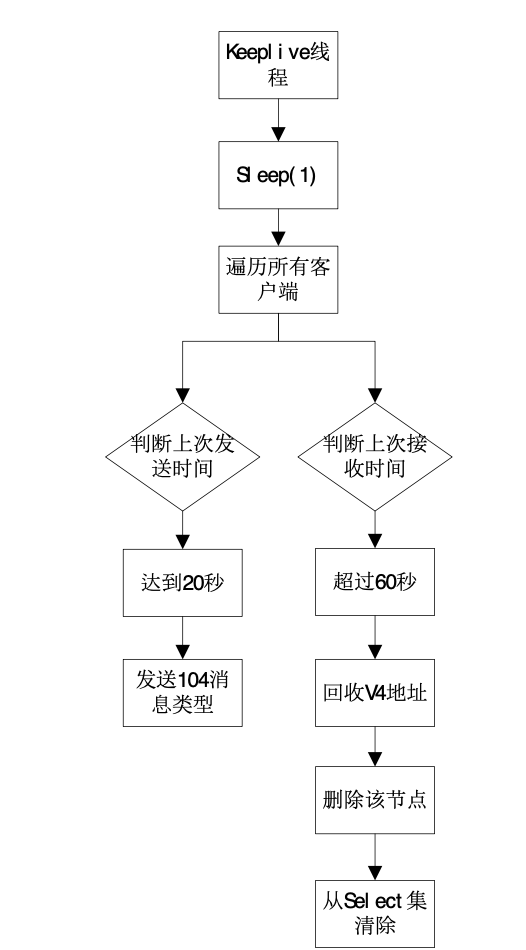
\includegraphics[scale=.58]{server_keep.png}
	\end{center}
	\caption{keeplive线程流程设计}
	\label{figure:keeplive线程流程设计}
\end{figure}

\section{服务器端具体实现}
服务器端大致思路在上述流程设计中已经叙述的足够清楚,在此不再赘述。本部分仅对关键技术要点(NAT、epoll和socket)进行叙述和讲解。
\subsection{NAT}
服务器端使用iptables做NAT,以此实现私有网段和公网地址之间的转换。
当一个客户端发起网络请求时,服务器端的iptables会进行"(客户端IP地址, 端口)即(Src IP, Src Port) -> (服务器端IP地址,端口)即(Dst IP, Dst Port)"之间的映射。 
当公网设备收到上述报文时,服务器端的iptables会根据端口号找到对应客户端的IP地址和监听端口,对该报文的目的地址和目的端口进行替换,这其实是一个逆映射过程。
这样,我们就完成了客户端到服务器端的NAT,实现了私有网段和公网地址之间的转换。

\subsection{epoll和socket}
和网上许多开源的服务器架构一样,我们的项目中,服务器端一样使用了非常便利好用的epoll函数,使用epoll函数同时监听所有客户端对应的socket。
当epoll函数监听到一个可用有效的socket的时候,我们首先会根据这个socket的描述符找到这个socket对应的客户端,然后执行相应的处理函数。
当epoll函数监听到其中任意一个socket状态为“可写”时,则从该客户端对应的数据队列里取出数据写入此socket,持续调用“write()”系统调用直到其返回“EAGAIN”(表明继续写入会导致阻塞),则停止写入。
若epoll函数监听到其中任意一个socket状态为“可读”时,则持续调用“read()”系统调用直到其返回“EAGAIN”(表明当前缓冲区里所有数据都已被读取)。若读到完整的消息,则去掉头部后直接写入隧道。 
我们的隧道同样是使用epoll函数进行监听,不同的是根据实现,每次对隧道调用“read/write”时都会“读/写”一个完整的IP包。从隧道中读到IP包后,则根据IP包头中的Dst IP找到对应的客户端,将该IP包放入对应客户端的数据队列中,待该用户的 socket 可用后发送。
通过上述实现,我们就完成了客户端与服务器端之间的socket连接与信息传输。
